\pagebreak
\section{Ejercicio 2}

\subsection{Problema: A Medias}
 Nos proveen la defici\'on de mediana de un conjunto ordenado de $n$ elementos como: \\
 $x_{(n+1)/2}$ si $n$ es impar \\
 $(x_{n/2} + x_{n/2+1)} /2$ si $n$ es par.\\
 
 Se nos pide dada una entrada de $n$ n\'umeros enteros no ordenados devolver otros $n$ n\'umeros donde el $i$\'esimo de ellos represente la parte entera de la funci\'on mediana aplicada a los primeros $i$ n\'umeros de la entrada, luego de ser ordenados. \\
 Adem\'as la resoluci\'on de este problema debe obtenerse en una complejidad estrictamente menor a $\bigO (n²)$ siendo $n$ el n\'umero total de enteros en la entrada.\\
 Luego, la entrada ser\'a una linea de $n$ n\'umeros, al igual que la salida.
\subsubsection{Ejemplos}


\begin{table}[htb]
\centering
\begin{tabular}{|l|l|}
\hline
Linea Entrada     & Linea Salida      \\ \hline
2 3 4 1 2         & 2 2 3 2 2         \\ \hline
2 7 2 8 4 9 1 6 5 & 2 4 2 4 4 5 4 5 5 \\ \hline
1 87 4            & 1 44 4            \\ \hline
4 0 32 6 8 10     & 4 2 4 5 6 7       \\ \hline
\end{tabular}
\caption{Ejemplos A Medias}
\label{my-label}
\end{table}

\subsection{Desarrollo} 
La complejidad intrinseca de este ejercicio esta en ir recorriendo un vector de n\'umeros, e ir de alguna manera ordenando este nuevo array para obtener f\'acilmente la mediana, que sabemos que si se cumple la anterior propiedad es muy f\'acil calcularlo. 
Para lograr esto hicimos uso de una estructura que nos permite obtener el valor del m\'inimo/m\'aximo barato y la insercion y borrado relativamente tambien.
La idea es mantener siempre la idea de puntero al medio de lo que seria el array actual, por lo que decidimos usar un minHeap, un maxHeap y una variable, lo que hace que nuestro array se convierta en la siguiente estructura. \\

\begin{center}
    [1 , 2 , 3 , 4 , 5] 
\end{center}\\

\begin{center}
    maxheap(1,2)  ++  3  ++ minHeap(4,5) 
\end{center}

La idea del "++"\ es que si vamos extrayendo el maxheap incrementando las posiciones , agregamos la variable del medio y luego extraemos el minHeap volvemos a obtener nuestro array inicial, este vendria a ser nuestro funcion de Abstraccion que matchea nuestra estructura con un array convencional.

Teniendo esta estructura es muy f\'acil ir agregando nuevos elementos y mantenerla consistente es muy sencillo. La idea es la siguiente:

Si el elemento nuevo es menor a la variable (esta es el "medio"), se agrega al maxHeap, caso contrario se la agrega al minHeap. Luego de esto se llama a una funcion que readjusta la estructura de ser necesario para luego simplemente, si el vector es de tama\~no par, se devuelve la suma de la variable mas el min/max del heap que tenga mas elementos, caso contrario se devuelve la variable.

Esta insercion puede generar la necesidad de ajustar la estructura, pero como veremos en la siguiente seccion esto a lo sumo necesita realizar dos pasos. 

\subsection{Justificaci\'on y Complejidad}
El algoritmo crea las estructuras necesarias para trabajar y son las siguientes. \\ \\ 
leftHeap \ \leftarrow \ maxHeap \ de\ tama$\~$no\ n \\
rigthHeap \ \leftarrow \ minHeap \ de\ tama$\~$no\ n \\
resultado  \ \leftarrow \ intArray \ de\ tama$\~$no\ n \\
middle \ \leftarrow intVariable \\

Luego tenemos un for que va a hacer las llamadas correspondientes para resolver el problema.

\begin{description}
    Algoritmo 2.1
    \begin{verbatim}
    FOR i desde 0 hasta n
        resultado[i] <- calcularMediana(array[i],i)
    ENDFOR
    \end{verbatim}   
\end{description}
Aca ya empezamos a observar que el costo de esta funcion al menos va a tener como cota $\bigO (n)$, ya que a lo sumo vamos a recorrer 1 vez el array entero pero nos falta analizar el costo de la funci\'on calcularMediana, por lo tanto la complejidad que podemos asegurar por ahora es $\bigO (n * \bigO(calcularMediana))$ \\ \\

Para analizar la funci\'on anterior vamos a dividirlo en 3 partes, pero antes debemos asegurarnos que las operaciones que utilicemos en los Heaps sean de la complejidad que afirmamos que son.

Para esto fuimos a la documentaci\'on oficial de oracle, en donde citamos la siguiente frase :

"Implementation note: this implementation provides O(log(n)) time for the enqueing and dequeing methods (offer, poll, remove() and add);"

Y la misma fue extraida del siguiente link:\\
\hypertarget{http://docs.oracle.com/javase/7/docs/api/java/util/PriorityQueue.html}

Luego de esta aclaracion podemos continuar con el analisis de las funciones, la interfaz de calculateMediana es :\\
int calculateMediana(int number, int i).


\begin{description}
  \item[Agregar nuevo elemento:] \hfill \\
  Esta seccion es la encargada de ingresar un nuevo elemento, para luego poder mas adelante calcular la mediana del array el cual deberiamos calcular. El pseudo-codigo es bastante sencillo, ya que tenemos un primer caso, en el cual no hay ningun elemento a\~nadido, es decir la estructura esta vacia, y por lo tanto la opreaci\'on simplemente consta en asignar la variable middle, caso contrario, debemos ver en que heap deberiamos insertar el elemento, sin temor a descompensar la estructura, ya que luego llamaremos a una funcion encargada de recomponer la misma de ser necesario.
Es importante observar que si ingresa un elemento repetido, y este es igual al middle, por como se armaron los casos, va a ir al rigthHeap, lo que no causaria ningun tipo de inconveniente. 


\begin{description}
    Algoritmo 2.2
  \begin{verbatim}
    IF i == 0 :
        middle <- number O(1) 
    ELSE :
        IF number < middle :
            leftHeap.add(number) // O(log(n))
        ELSE : 
            rigthHeap.add(number) // O(log(n))
        ENDIF 
    ENDIF
    \end{verbatim}
\end{description}
    
Por lo tanto podemos acotar esta seccion de la funci\'on con costo :  $\bigO (log(n))$
  \item[ajustar la estructura:] \hfill \\
  
  Esta seccion es la que se encarga de en otras palabras, hacer valer nuestro invariante de representacion, que es mantener la variable middle en lo que pasando por nuestra funcion de abstraccion es el centro del array, en caso de ser impar y sino uno de los dos elementos del "medio", en caso de ser par.
  
  El pseudo codigo de la funcion es el siguiente:

\begin{description}
    Algoritmo 2.3
  \begin{verbatim}
    IF rigthHeap.size() - leftHeap.size() > 1 :
        leftHeap.add(middle)   // O(log(n))
        middle = rigthHeap.remove()  // O(log(n)) 
    ELSE IF leftHeap.size() - rigthHeap.size() > 1 :
        rigthHeap.add(middle)  // O(log(n))
        middle = leftHeap.remove() // O(log(n))
    ENDIF
  \end{verbatim}
\end{description}
 
 Olvidandonos de que hay casos en los cuales, esta parte de la funcion tenga costo  $\bigO (1)$ \ ya que no entrariamos en ningun caso, si podemos asegurar que en el caso de necesitar relaizar un adjuste, solo vamos a realizar uno, esto se traduce a ejecutar una sola parte del if.
 Vamos a ver que por absurdo estas condiciones no pueden cumplirse simultaneamente:
 
 Sea a = rigthHeap.size() y b = leftHeap.size() .
 
 Asumimos que  : a - b > 1 y queremos llegar a que b - a > 1
 
 Podemos hacer un pasaje de terminos en la primera por lo que nos quedaria : a > b + 1
 
 Y de la segunda sabemos que b > a + 1, por lo tanto si juntamos las inecuaciones nos queda:
 
 b > a + 1 > a > b + 1  \ \   Abs! 
 
 Como llegamos al absurdo de que b > b + 1 podemos concluir que si sucede a - b > 1, no puede suceder b - a > 1 . Esto lo podemos hacer sin perdida de generalidad y vamos a llegar a la misma conclusion.
 
Por lo tanto este analisis no lleva a poder afirmar que una cota para esta seccion es $\bigO (2 * log(n))$, pero si nos lanzamos a calcular la complejidad sin ningun analisis, la complejidad estaria acotada por $\bigO (4 * log(n))$ y como 2 y 4 son constantes llegamos a la cota final de $ \textbf {\bigO (log(n))}$
 
	
  \item[Devolver el resultado:] \hfill \\
  En esta ultima seccion, lo unico que debemos es identificar en que caso de array estamos, es decir par o impar, por lo que el pseudo-codigo seria el siguiente:
\begin{description}
    Algoritmo 2.4
    \begin{verbatim}
        IF (i+1) % 2 == 0) :
            IF (rigthHeap.size() > leftHeap.size()) :
                return ((rigthHeap.peek() + middle) /2) // O(1)
            ELSE :
                return ((leftHeap.peek() + middle) /2) // O(1)
            ENDIF
        ELSE :
            return middle // O(1)
        ENDIF
    \end{verbatim}
\end{description}

La funcion peek, lo que hace es ver el min/max elemento, y esto lo hace en $\bigO (1)$, por lo tanto la complejidad final de esta seccion es $\textbf{\bigO (1)}$ para cualquier caso, de entrada posible.

\end{description}

Sumando todas las complejidades de las tres divisiones que hicimos, nos queda que la funcion calculateMediana tiene una complejidad de $\bigO (log(n))$ .

Al tener resuelta esta parte, podemos completar lo que antes no podiamos asegurar y por lo tanto la complejidad del problema es :\\

${\bigO (n * log(n))$ \\

Y como $\bigO (log(n))$ < $\bigO (n^2)$, podemos concluir que : \\

$\bigO (n * log(n))$ < $\bigO (n^2)$ \\

Por lo tanto nuestro algoritmo cumple con la complejidad pedida.

\pagebreak

\subsection{Correctitud}

Para empezar a mostrar la correctitud de nuestro algoritmo, vamos a escribir nuestro invariante de representacion en un pseudo lenguaje.

\begin{verbatim}
1) FOREACH leftHeap as element:
    element <= middle
ENDFOREACH
2) FOREACH rigthHeap as element:
    element >= middle
ENDFOREACH
3) | rigthHeap.size() - leftHeap.size()| < 2

\end{verbatim}

Suponiendo que este invariante de representacion, es muy f\'acil ver que la solucion va a hacer correcta, por la definicion de mediana.
Veamos que la definicion de mediana, es igual a nuestra funcion de calcular resultado.

\begin{table}[htb]
\centering
\begin{tabular}{|l|l|l|}
\hline
    & Solucion Mediana  &  Solucion Nuestra     \\ \hline
Caso PAR        & (x_{n/2} + x_{n+1/2})/2 &   ((rigthHeap.peek() + middle) /2) V    \\ 
 & &((leftHeap.peek() + middle) /2 ) \\ \hline
Caso IMPAR & x_{(n+1)/2} &   middle \\ \hline

\end{tabular}
\caption{Comparaci\'on de soluciones}
\label{my-label}
\end{table}

Para no ser redundantes con la copia del codigo, vamos a explicar brevemente que en el caso par, al no existir un "medio", nuestra estructura tiene en la variable middle, uno de los 2 "medios", y con observar el tama\~no de los heaps, podemos determinar cual de ellos tiene al otro "medio".

Ahora que sabemos que de nuestro invariante podemos llegar a la solucion pedida, nos queda ver que haciendo la unica operacion posible con este algotirmo que es agregar un nuevo elemento, la estructura sigue manteniendo el invariante al finalizar su ejecuci\'on.

Veamos primero nuestro case base, las estructuras vacias, y nuestra variable middle sin inicializar. Al no haber elementos en ninguno de los 2 heaps , el FOREACH se cumple trivialmente ya que no hay elementos para ver si la condicion que pedimos es valida. y el tercer punto tambien se cumple trivialmente, si no tiene elementos los tama\~nos son 0, por lo tanto la diferencia entre ellos es 0 y menor que 2.

Luego nos queda ver que pasa al agregar un nuevo elemento, la parte 1 y 2 del invariante de Representacion nunca deja de valer. En la seccion anterior, en la parte que titulamos "Agregar nuevo elemento" y que ser\'ia el Algoritmo 2.2 , vemos ese IF hace que los elementos nuevos se agregen respetando nuestros requerimientos, ya que seria la union de los 2 primeros puntos del invariante plasmados a las condiciones que utilizamos.

Nos falta ver que se sigue cumpliendo la tercera, y para esto nos vamos a apoyar en nuestra funcion de readjuste, que es Algoritmo 2.3. Comprobemoslo con un peque\~no ejemplo pero sin perder la generalidad de en que caso estemos.

Para esto vamos a suponer que nuestro variable middle vale j y vamos a agregar un nuevo elemento llamado k, sin perdida de generalidad podriamos suponer  que j < k y ahora tenemos que ver varios casos en los cuales los heaps tienen distintas cantidad de elementos. Para esto vamos a llamar a nuestro factor de balanceo como | rigthHeap.size() - leftHeap.size()| .

  
\begin{description}
\item[CASO 1, FACTOR DE BALANCEO 0:] \hfill \\
    Este caso es trivial, ya que si nuestro factor de balanceo es 0, agregando un elemento en cualquiera de los heaps, y luego recalculando nuestro factor va a hacer 1, por lo tanto menor a 2, es decir cumple el invariante de representacion.

\item[CASO 2, FACTOR DE BALANCEO 1:] \hfill \\
    Que nuestro factor de balanceo sea 1 significa que uno de los heaps tiene un elemento mayor que el otro, por lo tanto podemos llamarlo H. Y ahora nuevamente tenemos dos casos. que el elemento j haya sido agregado a H o no.
    
    
\begin{center}
\begin{description}
\item[CASO 1, j es agregado a H:] \hfill \\
    En este caso H ya tenia un elemento mas, y como le estamos agregando j, el factor de balanceo pasa a ser 2. por lo tanto lo que debemos hacer y lo que hace el algoritmo realiza es un balanceo. Por lo tanto nuestro algoritmo haria las siguientes acciones :
    
    Vamos a llamar a nuestro otro heap T, el distinto de H.
    \begin{verbatim}
    T.add(middle)   // O(log(n))
    middle = H.remove()  // O(log(n)) 
    \end{verbatim}
Por lo tanto podemos ver que antes de hacer estas dos operaciones estabamos en un factor de balanceo 2, pero agregamos un elemento en T y quitamos uno en H. Por lo tanto nuestro nuevo factor de balanceo en caso de haber hecho un rebalanceo pasa a ser de 0.
\item[CASO 1, j no es agregado a H:] \hfill \\
    Si H tenia un elemento mas pero agregamos un nuevo elemento en el heap T, es facil ver que el factor de balanceo vuelve a tener valor 0, por lo tanto no es necesario hacer ningun readjuste, ya que el elemeto mejora el factor por si solo.

\end{description}
\end{center}

\end{description}

factor de balanceo estaba en 1, lo que significa que uno de los 2 heaps, tenia un elemento mas que el otro, para el proposito de esta demostraci\'on vamos a suponer que este es el rigthHeap, ya que sino no se desbaleancearia la estructura, y no podriamos observar lo que queremos demostrar.



\begin{table}[htb]
\centering
\begin{tabular}{|l|l|l|l|l|}
\hline
    & Tama\~no leftHEAP & Tama\~no rigthHEAP  & valor Middle & Balanceo     \\ \hline
Antes de agregar       & 3  &  4 & 5 & 1       \\ \hline
Despues de agregar & 3 & 5 & 5& 2 \\ \hline

\end{tabular}
\label{my-label}
\end{table}

Si entramos a la funcion encargada de ajustar la estructura, es f\'acil notar que vamos a entrar en este if:
\begin{verbatim}
IF rigthHeap.size() - leftHeap.size() > 1 :
        leftHeap.add(middle)
        middle = rigthHeap.remove()
\end{verbatim}

Entonces volvamos a ver como nos queda nuestro cuadro luego de aplicar esta seccion de la funcion:

\begin{table}[htb]
\centering
\begin{tabular}{|l|l|l|l|l|}
\hline
    & Tama\~no leftHEAP & Tama\~no rigthHEAP  & valor Middle & Balanceo     \\ \hline

Despues de agregar & 3 & 5 & 5& 2 \\ \hline
Despues de ajustar & 4  &  4 & m\'inimo(rigthHeap) & 0      \\ \hline
\end{tabular}
\label{my-label}
\end{table}

Hay que destacar que m\'inimo(rigthHeap) es el elemento m\'inimo que se extrajo en el algoritmo, y por eso su tama\~no bajo en 1. 

Luego vemos que la tercera parte del invariante se cumple, sin perder generalidad podemos ver que como en cada iteracion se llama a esta funcion y solo se agrega a un elemento a la vez, nunca vamos a tener una diferencia mayor a 2, por lo tanto el adjuste de mover un elemento desde el que mas tiene hasta el que menos tiene, teniendo el cuidado de hacer la transicion correspondiente para mantener el punto 1 y 2, balancea la estructura y mantiene los tres puntos de nuestro invariante.

Al haber probado que :
\begin{itemize}
\item Una estructura que cumple el invariante de representacion podemos ir a la solucion del problema.
\item Al agregar un elemento a una instancia que cumple el invariante de representacion, nos lleva a otra instancia valida con ese elemento.
\end{itemize}

Podemos concluir que al agregar un nuevo elemento podemos llegar a una instancia valida, que luego podremos convertirla en una solucion del problema.


\subsection{Tests}
Para los Tests analizamos su mejor y peor caso.
    \subsubsection{Mejor Caso}
        El mejor caso es que el primer elemento se el elemento del medio y que la distribucion de la entrada sea (<middle),(>middle),(<middle) ... lo que va a generar que nunca se necesite balancear la estructura quedando cada iteracion con el costo de insertar un nuevo elemento en un heap, y eso nos cuesta: $\bigO(log(n))$. \newline
    \lstinputlisting[language=Java]{modulos/Tests_Code/testej2mejor.txt}
    \subsubsection{Peor Caso}
        El peor caso es cuando la distribucion de la entrada es monotona creciente/decreciente lo que generaria la necesidad de reajustar la estructura siempre luego de la segunda iteracion, y recordemos que el adjuste de la estructura nos cuenta $\bigO(2 * log(n))$ y a esto hay que sumarle el costo que tenemos siempre de agregar el elemento para luego revisar si hay que rebalancear que es $\bigO(log(n))$ , lo que nos da un total de $\bigO(3 *log(n))$ para cada iteracion luego de la segunda.. \newline
 \lstinputlisting[language=Java]{modulos/Tests_Code/testej2peor.txt}
 
\pagebreak

\subsubsection{Performance}

Comparaci\'on de mejor peor caso. Vemos que crecen asint\'oticamente igual, s\'olo que con distintas pendientes. La constante 3 que afecta al peor caso, surge de que en este caso se suma a la misma inserci\'on del mejor caso, dos mas que son causa de mover el middle a un heap, y el heap que tenia mas elementos a middle.

\begin{figure}[h!]
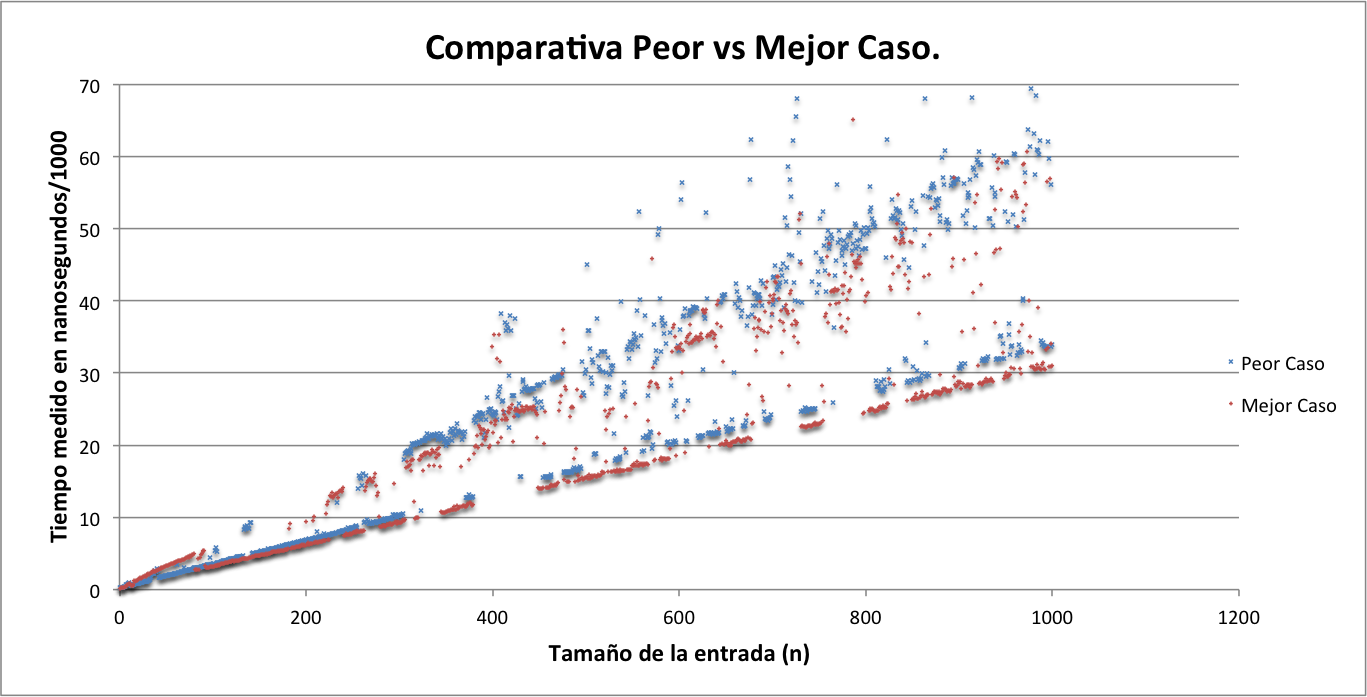
\includegraphics[width=140mm]{ejercicio2_bestVsworst.png}
\centering
\caption{Comparativa Peor vs Mejor Caso}
\label{overflow3}
\end{figure}


Luego podemos ver que la cota que justificamos como  $\bigO(n * log(n))$ est\'a acotada inferiormente por una funci\'on lineal a partir de un n.


\begin{figure}[h!]
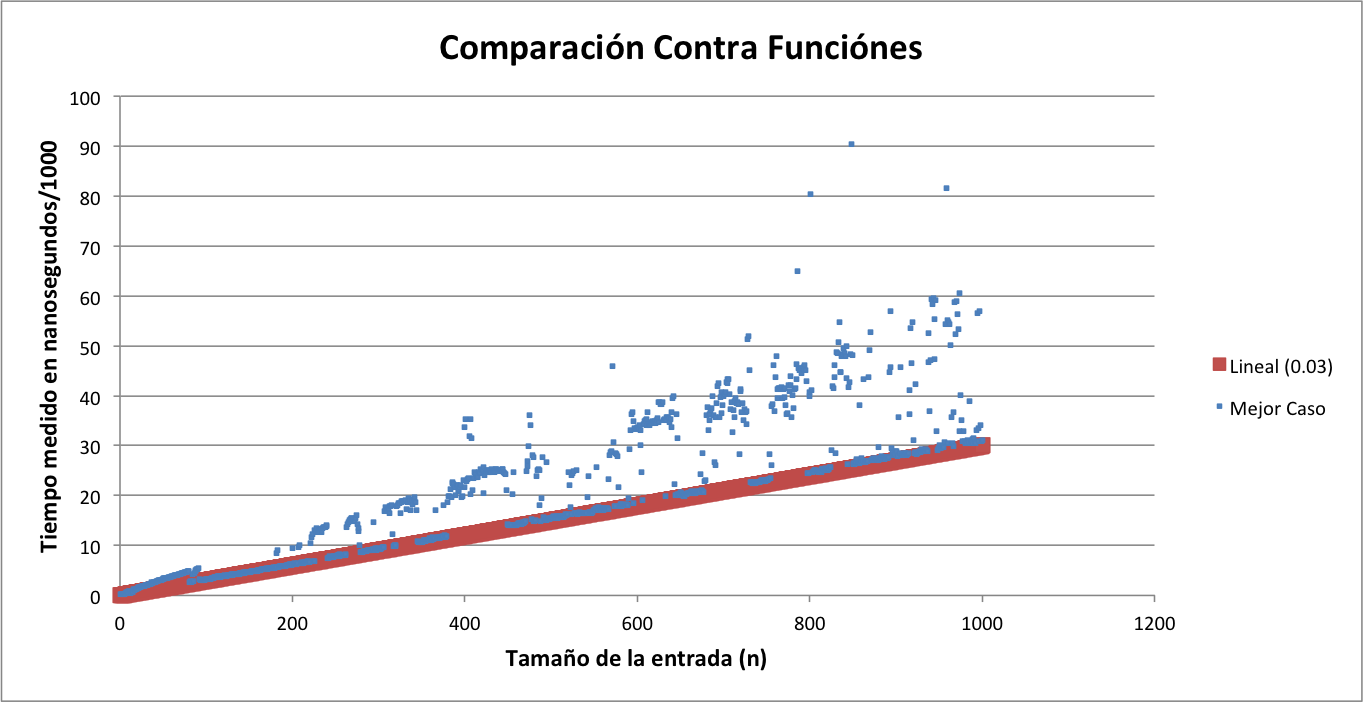
\includegraphics[width=140mm]{ejercicio2_comparacionvsfunciones.png}
\centering
\caption{Comparativa Contra Funcion Lineal y Cuadratica}
\label{overflow3}
\end{figure}

